\documentclass[border=6pt]{standalone}
\usepackage{amsmath}
\usepackage{amssymb}
\usepackage{tikz}
\usepackage{pgfplots}
\pgfplotsset{compat=1.18}
\usetikzlibrary{arrows.meta,calc,positioning}
\begin{document}
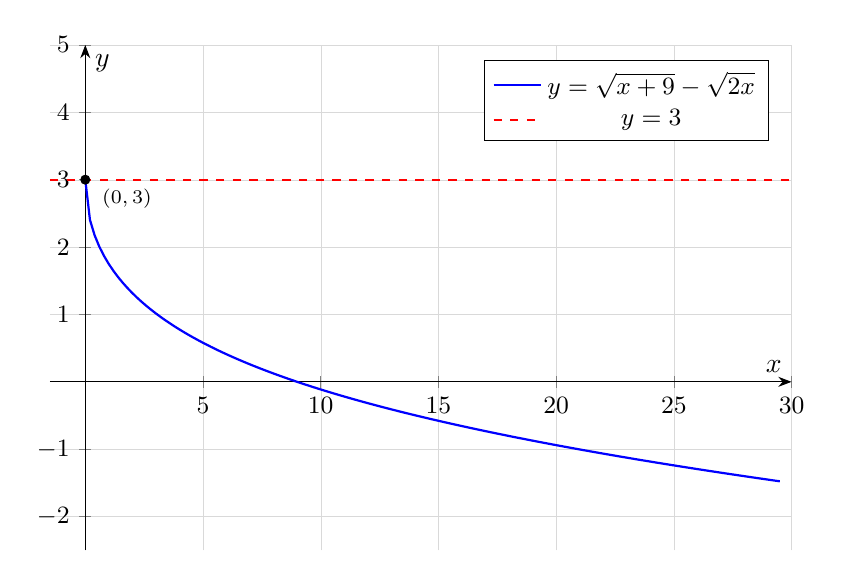
\begin{tikzpicture}
\begin{axis}[
    axis lines = middle,
    xlabel = {$x$}, ylabel = {$y$},
    grid=both,
    grid style={line width=.1pt, draw=gray!30},
    axis line style={-Stealth},
    legend style={font=\small},
    tick label style={font=\small},
    xmin=-1.5, xmax=30, ymin=-2.5, ymax=5,
    xtick={0,5,10,15,20,25,30},
    ytick={-2,-1,0,1,2,3,4,5},
    width=11cm, height=8cm,
    legend pos=north east,
]
\addplot[domain=0:29.5, samples=150, thick, blue] {sqrt(x+9)-sqrt(2*x)};
\addlegendentry{$y=\sqrt{x+9}-\sqrt{2x}$}
\addplot[domain=-1.5:30, samples=2, thick, red, dashed] {3};
\addlegendentry{$y=3$}
\addplot[only marks, mark=*, mark size=1.6pt, black] coordinates {(0,3)};
\node[anchor=north west, font=\scriptsize] at (axis cs:0.3,3) {$(0,3)$};
\end{axis}
\end{tikzpicture}
\end{document}
